% ============================================================
% Project 2 Report — Neural Network and Deep Learning
% ============================================================
\documentclass[11pt,a4paper]{article}

% ---------- Packages ----------
\usepackage[utf8]{inputenc}
\usepackage[T1]{fontenc}
\usepackage{amsmath,amssymb}
\usepackage{graphicx}
\usepackage{booktabs}
\usepackage{hyperref}
\usepackage{geometry}
\usepackage{float}
\usepackage{caption}
\usepackage{subcaption}
\usepackage{enumitem}
\usepackage[table]{xcolor}
\usepackage{multirow}
\usepackage{array}

\geometry{margin=1in}
\hypersetup{
    colorlinks=true,
    linkcolor=blue,
    urlcolor=blue,
    citecolor=blue
}

% ---------- Title ----------
\title{\textbf{Project 2: Neural Network Training on CIFAR-10\\[4pt]
        and Batch Normalization Analysis}}
\author{
    \textbf{Name:} \texttt{Qilin Jin} \quad
    \textbf{Student ID:} \texttt{23307110152} \\[6pt]
    \textbf{GitHub:} \url{https://github.com/KylinKingI/CS30064.01-pj2} \\[4pt]
}
\date{May 8, 2026}

\begin{document}
\maketitle

% ============================================================
% 1. Train a Network on CIFAR-10
% ============================================================
\section{Train a Network on CIFAR-10}
\label{sec:cifar10}

\subsection{Dataset and Experimental Setup}

CIFAR-10~\cite{krizhevsky2009learning} is a widely-used benchmark dataset for image classification. It contains 60,000 $32\times32$ color images evenly distributed across 10 classes: airplane, automobile, bird, cat, deer, dog, frog, horse, ship, and truck. The dataset is split into 50,000 training images and 10,000 test images.

In our experiments, we use the following data preprocessing and augmentation pipeline:
\begin{itemize}[nosep]
    \item Normalization: mean = (0.5, 0.5, 0.5), std = (0.5, 0.5, 0.5)
    \item Training augmentation: RandomHorizontalFlip, RandomCrop (32$\times$32 with padding=4), ColorJitter (brightness=0.1, contrast=0.1)
    \item Batch size: 128
    \item Training epochs: 50
    \item Learning rate scheduler: CosineAnnealingLR
    \item Random seed: 42 (for reproducibility)
\end{itemize}

All experiments are implemented in PyTorch and run on a GPU when available.

\subsection{Network Architecture: CNN\_Residual}

All experiments in Part~1 use the \textbf{CNN\_Residual} architecture—a convolutional neural network that combines Batch Normalization with residual connections. This single architecture was chosen because it naturally satisfies all the required and optional component constraints of the project within one unified design. Rather than comparing different architectures, our experimental methodology focuses on systematically varying individual hyperparameters while holding the base architecture fixed, allowing us to isolate the effect of each parameter on performance.

\paragraph{Architecture Details.} CNN\_Residual consists of three convolutional stages followed by a classifier:

\begin{itemize}[nosep]
    \item \textbf{Stage 1:} Conv2d(3, $c_1$, 3$\times$3) $\rightarrow$ BN $\rightarrow$ Activation $\rightarrow$ ResBlock($c_1$) $\rightarrow$ MaxPool(2)
    \item \textbf{Stage 2:} Conv2d($c_1$, $c_2$, 3$\times$3) $\rightarrow$ BN $\rightarrow$ Activation $\rightarrow$ ResBlock($c_2$) $\rightarrow$ MaxPool(2)
    \item \textbf{Stage 3:} Conv2d($c_2$, $c_3$, 3$\times$3) $\rightarrow$ BN $\rightarrow$ Activation $\rightarrow$ ResBlock($c_3$) $\rightarrow$ MaxPool(2)
    \item \textbf{Classifier:} FC($c_3$$\times$4$\times$4, $f_1$) $\rightarrow$ Activation $\rightarrow$ FC($f_1$, $f_2$) $\rightarrow$ Activation $\rightarrow$ FC($f_2$, 10)
\end{itemize}

Each ResBlock consists of two Conv+BN layers with a skip (identity) connection:
$\text{out} = \text{Activation}(\text{Conv-BN-Conv-BN}(x) + x)$.

The channel dimensions default to $(c_1, c_2, c_3) = (64, 128, 256)$ and hidden FC dimensions to $(f_1, f_2) = (256, 128)$. These are scaled by a \texttt{width} multiplier for capacity experiments.

\subsubsection{Required and Optional Components}

Table~\ref{tab:components} shows how CNN\_Residual satisfies the project's component requirements. All four required components are integral to the architecture, and two optional components—Batch Normalization and Residual Connections—are built in. This allows us to conduct all experiments on a single, well-engineered baseline.

\begin{table}[H]
\centering
\caption{Components of CNN\_Residual and their correspondence to project requirements.}
\label{tab:components}
\begin{tabular}{@{}lll@{}}
\toprule
\textbf{Category} & \textbf{Component} & \textbf{Location in CNN\_Residual} \\
\midrule
\multirow{4}{*}{Required (all)}
    & Fully-Connected layer      & 3-layer classifier head \\
    & 2D Convolutional layer     & Conv layers in projection + ResBlocks \\
    & 2D Pooling layer (MaxPool) & After each stage \\
    & Activations                & After every Conv and FC layer \\
\midrule
\multirow{2}{*}{Optional ($\ge$1)}
    & Batch Normalization        & After every Conv layer \\
    & Residual Connection        & Skip connection in each ResBlock \\
\bottomrule
\end{tabular}
\end{table}

\subsection{Optimization Strategy: Controlled Parameter Sweeps}

Our experimental methodology follows a \textbf{controlled-variable} approach: we start from a baseline configuration of CNN\_Residual and vary one parameter at a time while keeping all others fixed. This allows us to isolate each parameter's contribution to performance. The baseline configuration is:

\begin{center}
\texttt{CNN\_Residual + ReLU + Adam + CrossEntropyLoss + width=1.0 + weight\_decay=$10^{-4}$}
\end{center}

The parameters we systematically explore are: (a)~number of neurons/filters (via the width multiplier), (b)~loss functions with different regularization strengths, (c)~activation functions, and (d)~optimizers. All experiments use a CosineAnnealingLR scheduler over 50 epochs with batch size 128.

\subsubsection{(a) Different Numbers of Neurons/Filters}

We vary the \texttt{width} multiplier $\in \{0.25, 0.5, 1.0, 1.5\}$, which scales all channel and hidden dimensions proportionally. All other hyperparameters (ReLU, Adam, CrossEntropyLoss, weight\_decay=$10^{-4}$) are held constant.

\begin{table}[H]
\centering
\caption{Effect of network width (number of neurons/filters) on classification performance.}
\label{tab:width}
\begin{tabular}{@{}lccc@{}}
\toprule
\textbf{Width} & \textbf{Parameters} & \textbf{Best Val Acc} & \textbf{Test Acc} \\
\midrule
0.25 & 189,258  & 0.8727 & 0.8727 \\
0.5  & 753,290  & 0.9099 & 0.9099 \\
1.0  & 3,005,706 & 0.9266 & 0.9266 \\
1.5  & 6,757,258 & 0.9303 & \textbf{0.9303} \\
\bottomrule
\end{tabular}
\end{table}

\textbf{Analysis:} Increasing width monotonically improves accuracy, but with clear diminishing returns. The jump from width~0.5 to 1.0 (+1.67\%) is substantially larger than from 1.0 to 1.5 (+0.37\%), despite the latter adding 3.75M more parameters. Width~1.0 (3.0M params) provides the best accuracy-efficiency trade-off, while width~1.5 (6.76M params) yields the highest raw accuracy at 93.03\%.

\subsubsection{(b) Different Loss Functions and Regularization}

We compare CrossEntropyLoss (CE) against CrossEntropyLoss with label smoothing ($\epsilon=0.1$), and further vary the $L_2$ regularization strength (weight\_decay $\in \{0, 10^{-4}, 10^{-3}\}$). All other parameters (CNN\_Residual, ReLU, Adam, width=1.0) are fixed.

\begin{table}[H]
\centering
\caption{Effect of loss function and weight decay (regularization) on test accuracy.}
\label{tab:loss}
\begin{tabular}{@{}lcc@{}}
\toprule
\textbf{Loss Function} & \textbf{Weight Decay} & \textbf{Test Acc} \\
\midrule
CrossEntropyLoss & 0.0            & 0.9236 \\
CrossEntropyLoss & $10^{-4}$      & 0.9266 \\
CrossEntropyLoss & $10^{-3}$      & 0.9227 \\
CE + Label Smoothing (0.1) & $10^{-4}$ & \textbf{0.9304} \\
CE + Label Smoothing (0.1) & $10^{-3}$ & 0.9219 \\
\bottomrule
\end{tabular}
\end{table}

\textbf{Analysis:} Label smoothing with $\epsilon=0.1$ provides the single largest improvement, boosting accuracy from 92.66\% to 93.04\%. This suggests it effectively prevents overconfidence and improves generalization. For weight decay, $10^{-4}$ is optimal: removing it entirely (wd=0) drops accuracy to 92.36\%, while increasing it to $10^{-3}$ over-regularizes (92.27\%). The combination of label smoothing + moderate weight decay ($10^{-4}$) yields the best result.

\subsubsection{(c) Different Activation Functions}

We compare ReLU, LeakyReLU ($\alpha=0.1$), and GELU. All other parameters (CNN\_Residual, Adam, CrossEntropyLoss, width=1.0, weight\_decay=$10^{-4}$) are fixed.

\begin{table}[H]
\centering
\caption{Effect of activation function on test accuracy.}
\label{tab:activation}
\begin{tabular}{@{}lcc@{}}
\toprule
\textbf{Activation} & \textbf{Parameters} & \textbf{Test Acc} \\
\midrule
ReLU                    & 3,005,706 & 0.9266 \\
LeakyReLU ($\alpha$=0.1) & 3,005,706 & 0.9252 \\
GELU                    & 3,005,706 & \textbf{0.9271} \\
\bottomrule
\end{tabular}
\end{table}

\textbf{Analysis:} All three activations perform within a narrow band (92.52\%--92.71\%), demonstrating that CNN\_Residual is robust to the choice of activation. GELU marginally leads (92.71\%), followed by ReLU (92.66\%) and LeakyReLU (92.52\%). Given ReLU's computational simplicity and nearly identical performance, it is the most practical choice.

\subsubsection{(d) Different Optimizers}

We compare Adam and Momentum SGD (momentum=0.9). Both use learning rate 0.01 with weight\_decay=$10^{-4}$. All other parameters (CNN\_Residual, ReLU, CrossEntropyLoss, width=1.0) are fixed.

\begin{table}[H]
\centering
\caption{Effect of optimizer on test accuracy.}
\label{tab:optimizer}
\begin{tabular}{@{}lcc@{}}
\toprule
\textbf{Optimizer} & \textbf{Learning Rate} & \textbf{Test Acc} \\
\midrule
Adam          & 0.01 & \textbf{0.9266} \\
Momentum SGD  & 0.01 & 0.9209 \\
\bottomrule
\end{tabular}
\end{table}

\textbf{Analysis:} Adam outperforms Momentum SGD by 0.57 percentage points. Its adaptive per-parameter learning rates provide faster and more stable convergence for the residual architecture on this dataset.

\subsection{Best Model and Final Results}

Across all experiments, the best-performing configuration achieves \textbf{93.04\% test accuracy} (test error = \textbf{6.96\%}):

\begin{itemize}[nosep]
    \item \textbf{Architecture:} CNN\_Residual (3 stages, residual blocks + BatchNorm)
    \item \textbf{Width:} 1.0 (3,005,706 parameters)
    \item \textbf{Activation:} ReLU
    \item \textbf{Optimizer:} Adam (lr=0.01, weight\_decay=$10^{-4}$)
    \item \textbf{Loss:} CrossEntropyLoss with label smoothing ($\epsilon$=0.1)
    \item \textbf{Scheduler:} CosineAnnealingLR
    \item \textbf{Epochs:} 50
\end{itemize}

The width=1.5 variant achieves nearly identical performance (93.03\%) but with over twice the parameters (6.76M), confirming that width=1.0 represents the optimal accuracy-efficiency trade-off. Table~\ref{tab:all_results} consolidates all experimental results for easy comparison.

\begin{table}[H]
\centering
\caption{Complete results of all CNN\_Residual experiments. The baseline configuration is highlighted in gray.}
\label{tab:all_results}
\begin{tabular}{@{}llllllc@{}}
\toprule
\textbf{Experiment} & \textbf{Width} & \textbf{Act.} & \textbf{Optim.} & \textbf{Loss} & \textbf{WD} & \textbf{Test Acc} \\
\midrule
\rowcolor{gray!15} Baseline & 1.0 & ReLU & Adam & CE & $10^{-4}$ & 0.9266 \\
\midrule
\multirow{3}{*}{Width} & 0.25 & ReLU & Adam & CE & $10^{-4}$ & 0.8727 \\
                        & 0.5  & ReLU & Adam & CE & $10^{-4}$ & 0.9099 \\
                        & 1.5  & ReLU & Adam & CE & $10^{-4}$ & \textbf{0.9303} \\
\midrule
\multirow{4}{*}{Loss / Reg.} & 1.0 & ReLU & Adam & CE & 0.0      & 0.9236 \\
                              & 1.0 & ReLU & Adam & CE & $10^{-3}$ & 0.9227 \\
                              & 1.0 & ReLU & Adam & CE+LS & $10^{-4}$ & \textbf{0.9304} \\
                              & 1.0 & ReLU & Adam & CE+LS & $10^{-3}$ & 0.9219 \\
\midrule
\multirow{2}{*}{Activation} & 1.0 & LeakyReLU & Adam & CE & $10^{-4}$ & 0.9252 \\
                             & 1.0 & GELU      & Adam & CE & $10^{-4}$ & \textbf{0.9271} \\
\midrule
Optimizer & 1.0 & ReLU & SGD+M & CE & $10^{-4}$ & 0.9209 \\
\bottomrule
\end{tabular}
\end{table}

\subsection{Network Insights and Visualization}

\subsubsection{Learning Curves}

Figure~\ref{fig:learning_curves} shows the training dynamics of our best model. The training loss decreases smoothly, and validation accuracy saturates around epoch~40, indicating that 50 epochs with cosine annealing provides sufficient training without significant overfitting. The gap between training and validation accuracy remains small throughout, demonstrating good generalization due to the combination of BatchNorm, label smoothing, and moderate weight decay.

\begin{figure}[H]
\centering
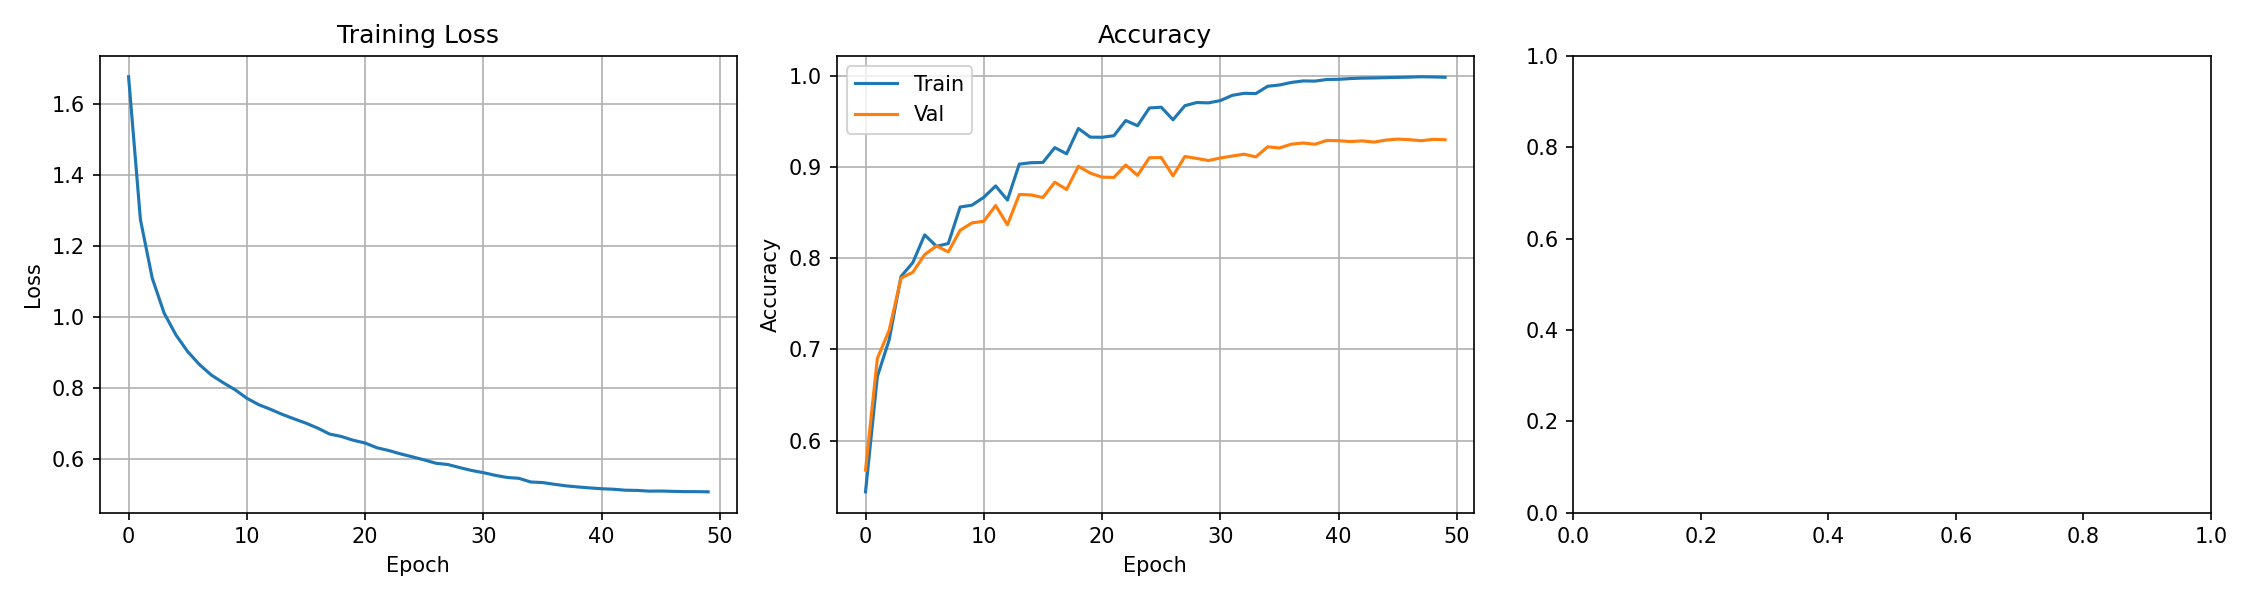
\includegraphics[width=0.95\textwidth]{codes/CIFAR10_CNN/saved/cnn_residual_relu_adam_ce_smooth_wd0.0001_wid1.0/cnn_residual_relu_adam_ce_smooth_wd0.0001_wid1.0_learning_curve.png}
\caption{Learning curves of the best model (CNN\_Residual, ReLU, Adam, Label Smoothing, width=1.0). Left: Training loss. Center: Training and validation accuracy over 50 epochs.}
\label{fig:learning_curves}
\end{figure}

\subsubsection{Convolutional Filter Visualization}

Figure~\ref{fig:filters} visualizes the first-layer convolutional filters of our best model. The filters exhibit diverse patterns including edge detectors at various orientations, color blobs, and texture-sensitive kernels. This diversity indicates that the network has learned a rich set of low-level feature extractors suitable for CIFAR-10 classification.

\begin{figure}[H]
\centering
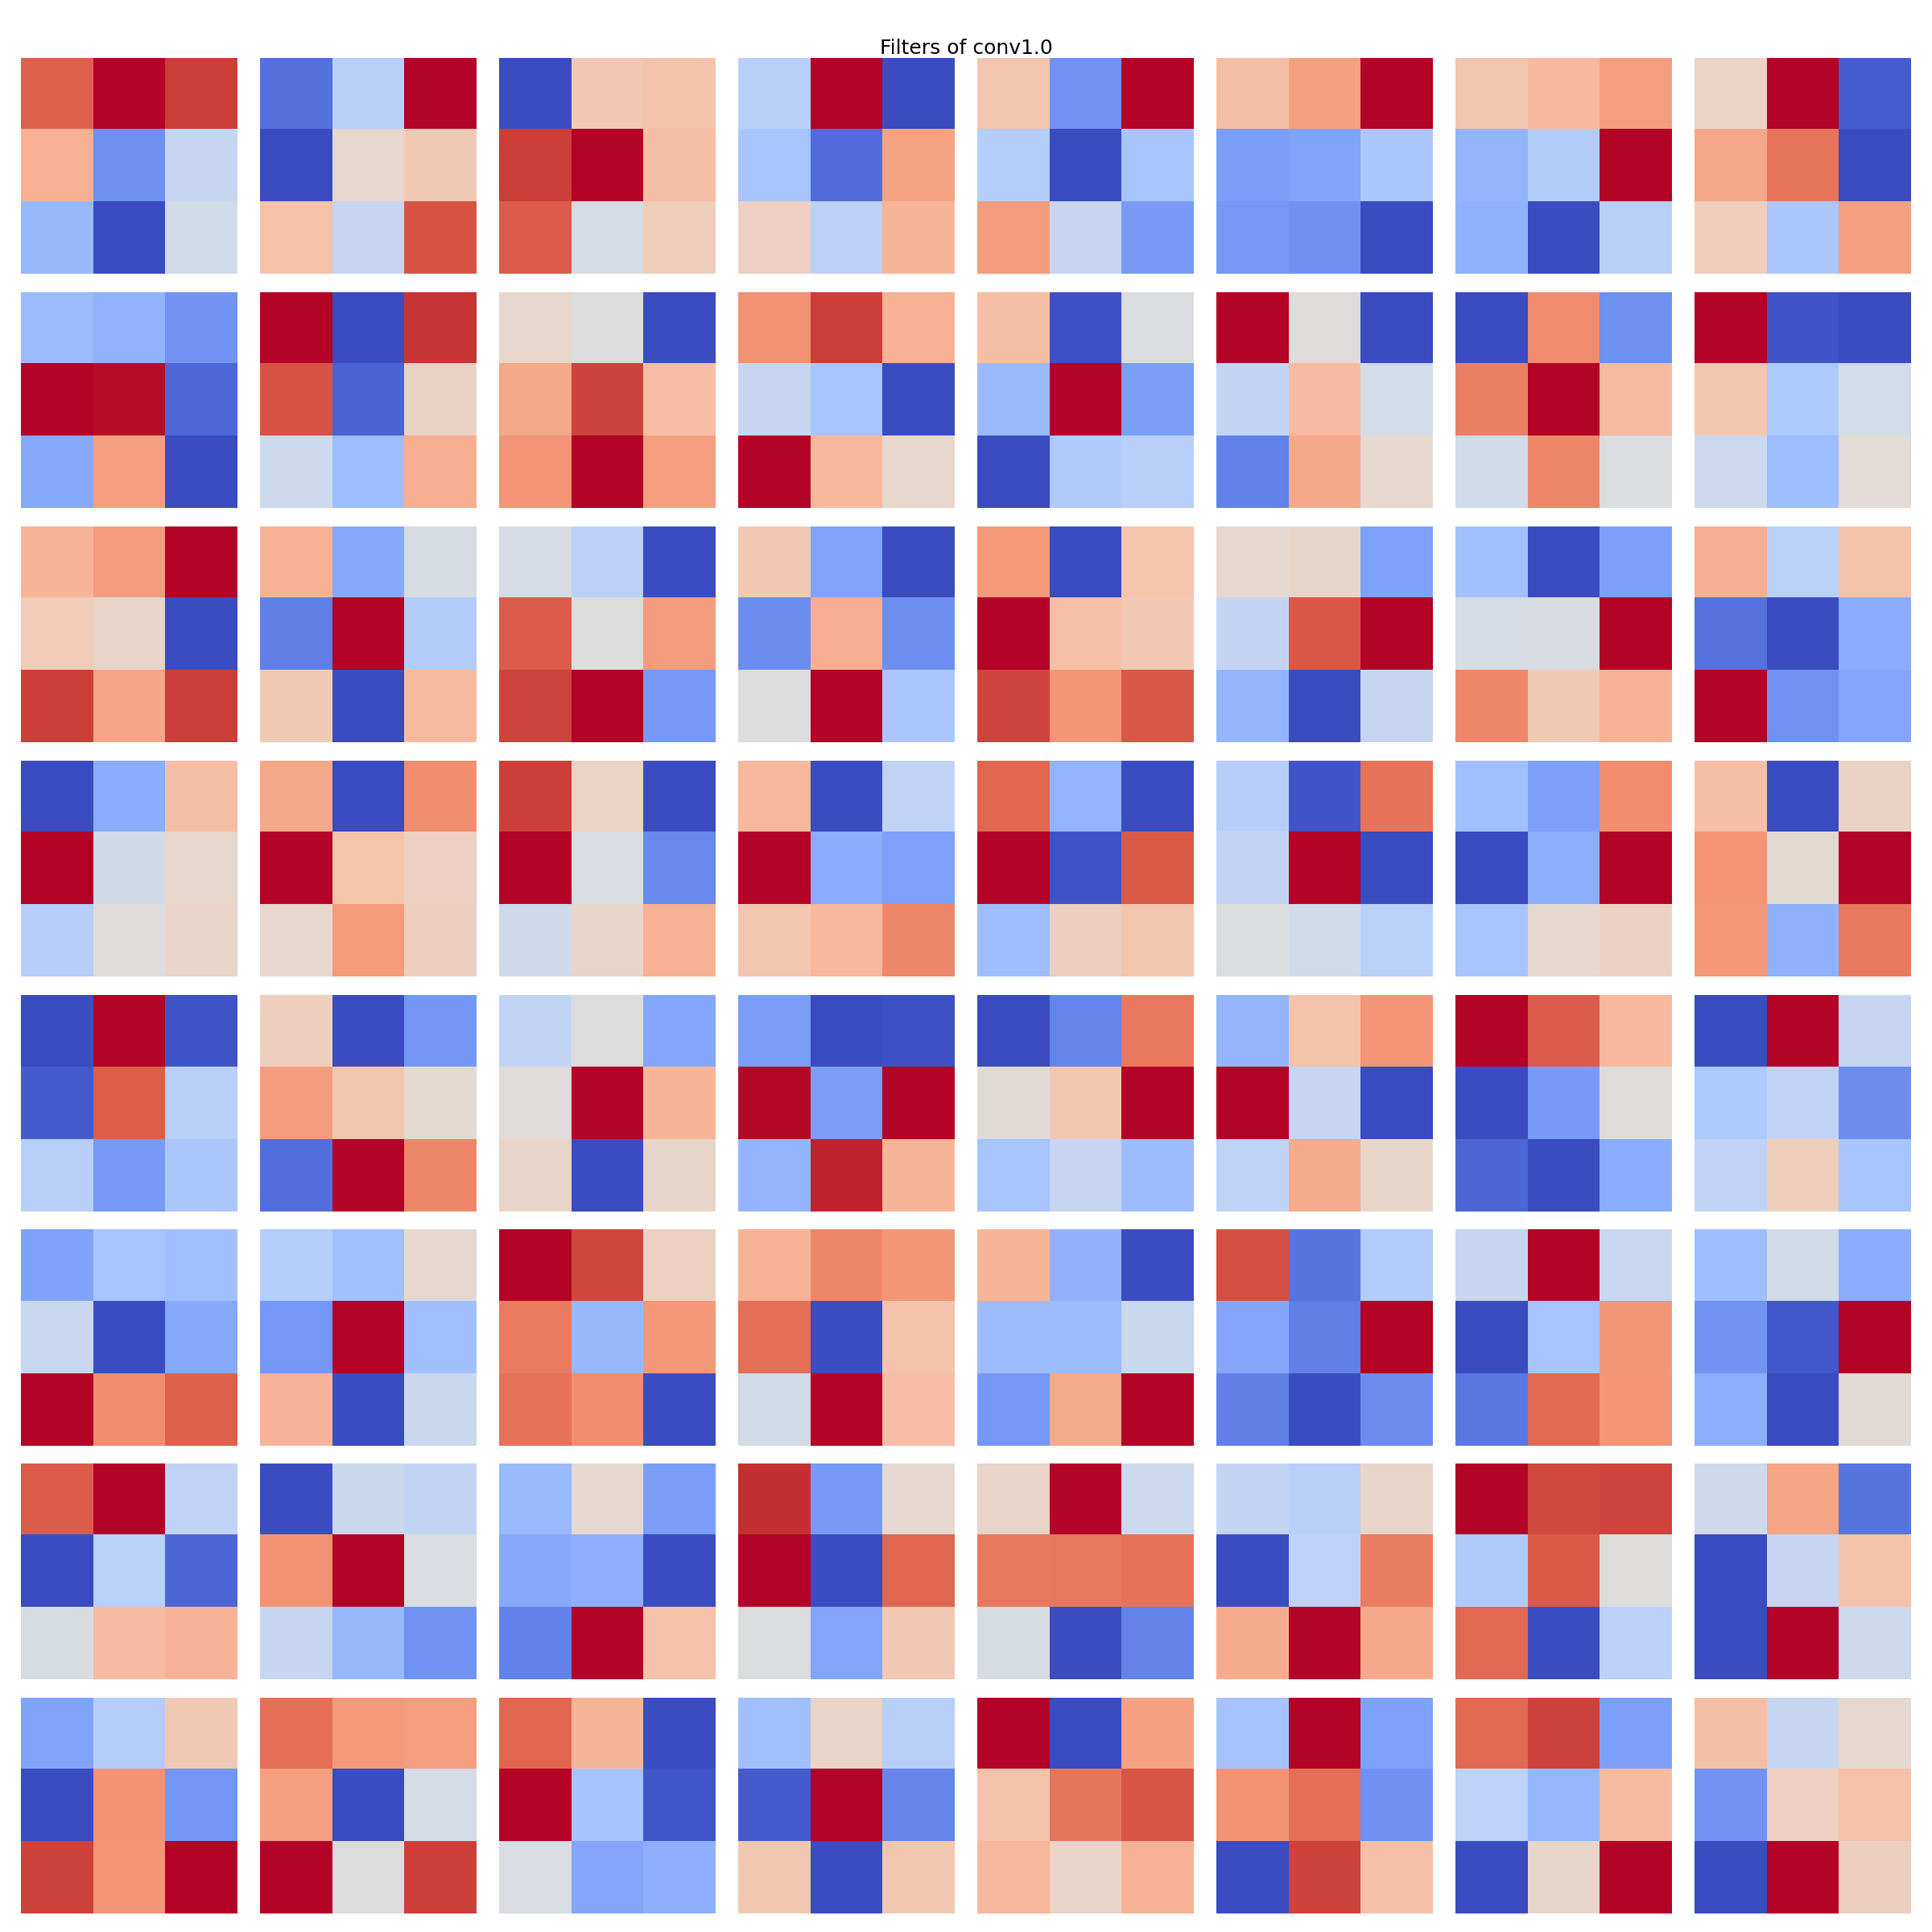
\includegraphics[width=0.7\textwidth]{codes/CIFAR10_CNN/saved/cnn_residual_relu_adam_ce_smooth_wd0.0001_wid1.0/cnn_residual_relu_adam_ce_smooth_wd0.0001_wid1.0_conv_filters.png}
\caption{Visualization of the first convolutional layer filters (64 channels). Filters show diverse edge and color detectors.}
\label{fig:filters}
\end{figure}

\subsubsection{Confusion Matrix}

Figure~\ref{fig:confusion} presents the confusion matrix on the test set. The model performs best on ``automobile'' and ``truck'' (well-separated classes), and struggles most with ``cat'' vs.~``dog'' and ``deer'' vs.~``horse''---pairs that share similar visual features even for humans.

\begin{figure}[H]
\centering
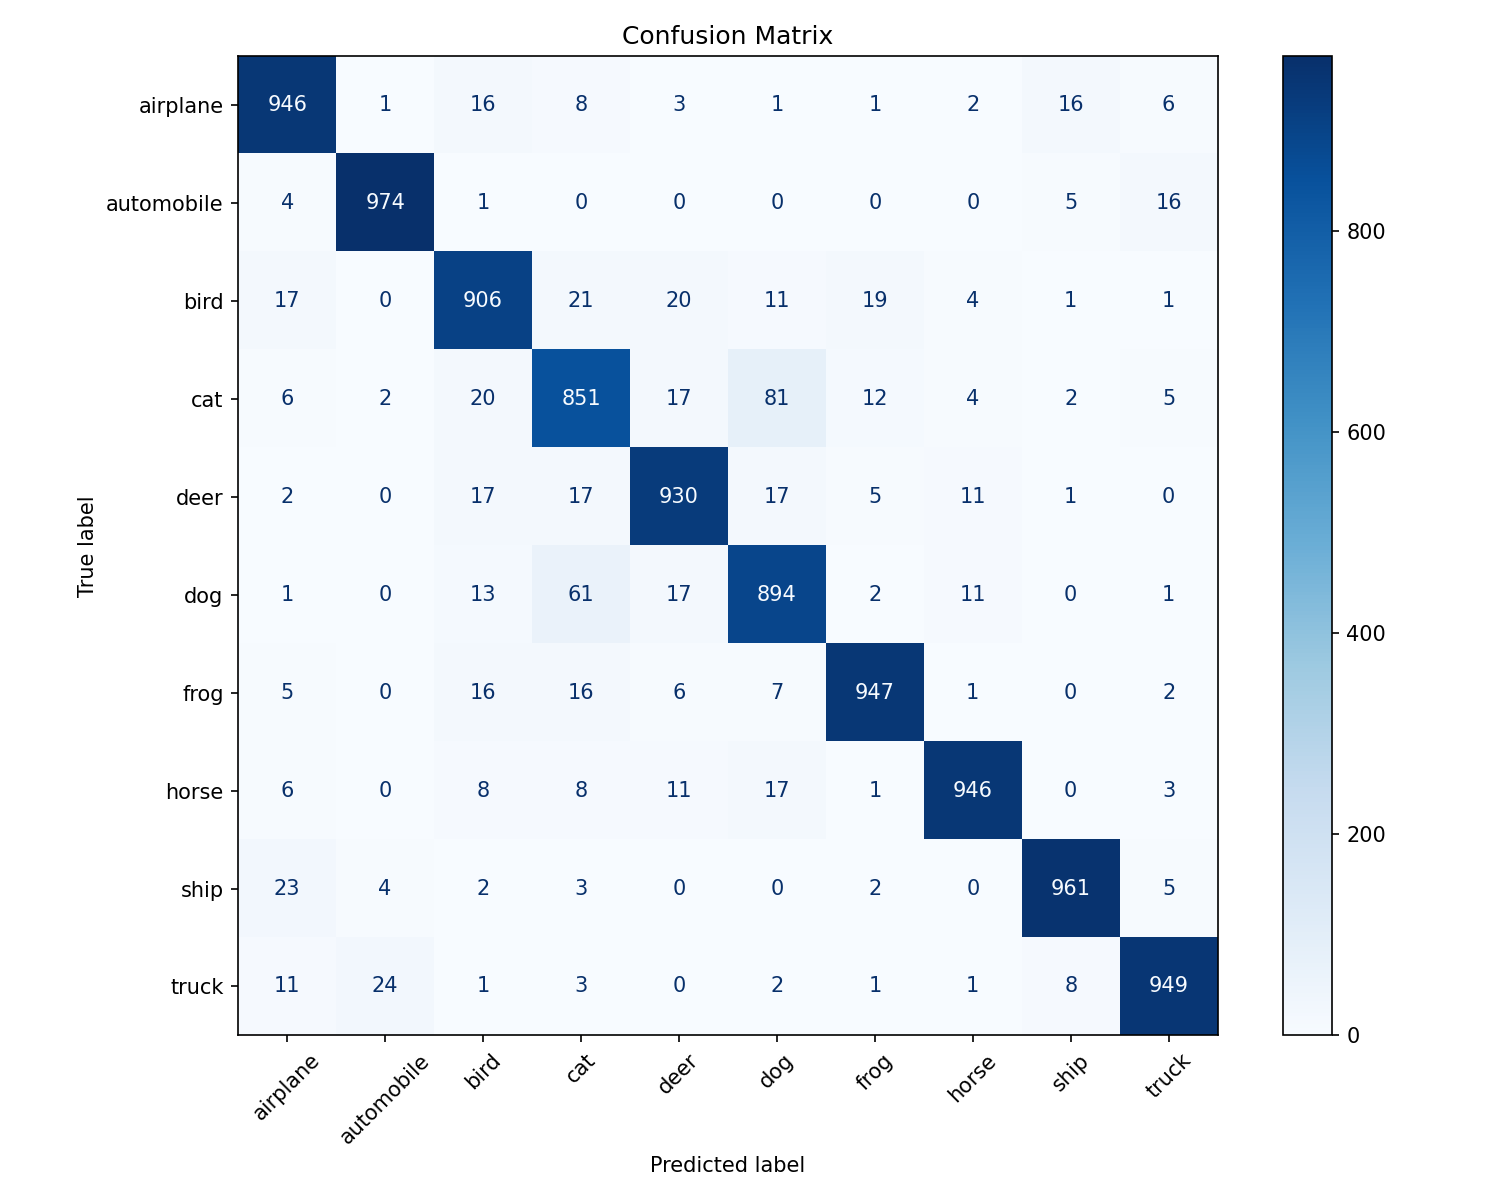
\includegraphics[width=0.65\textwidth]{codes/CIFAR10_CNN/saved/cnn_residual_relu_adam_ce_smooth_wd0.0001_wid1.0/cnn_residual_relu_adam_ce_smooth_wd0.0001_wid1.0_confusion_matrix.png}
\caption{Confusion matrix on the CIFAR-10 test set. The diagonal dominates, confirming strong classification performance.}
\label{fig:confusion}
\end{figure}

\subsubsection{Misclassified Examples}

Figure~\ref{fig:misclassified} shows 16 misclassified test examples with their true and predicted labels. Common failure modes include: (1) visually similar animal pairs (cat $\leftrightarrow$ dog, deer $\leftrightarrow$ horse), (2) low-contrast or ambiguous images, and (3) objects photographed from unusual angles.

\begin{figure}[H]
\centering
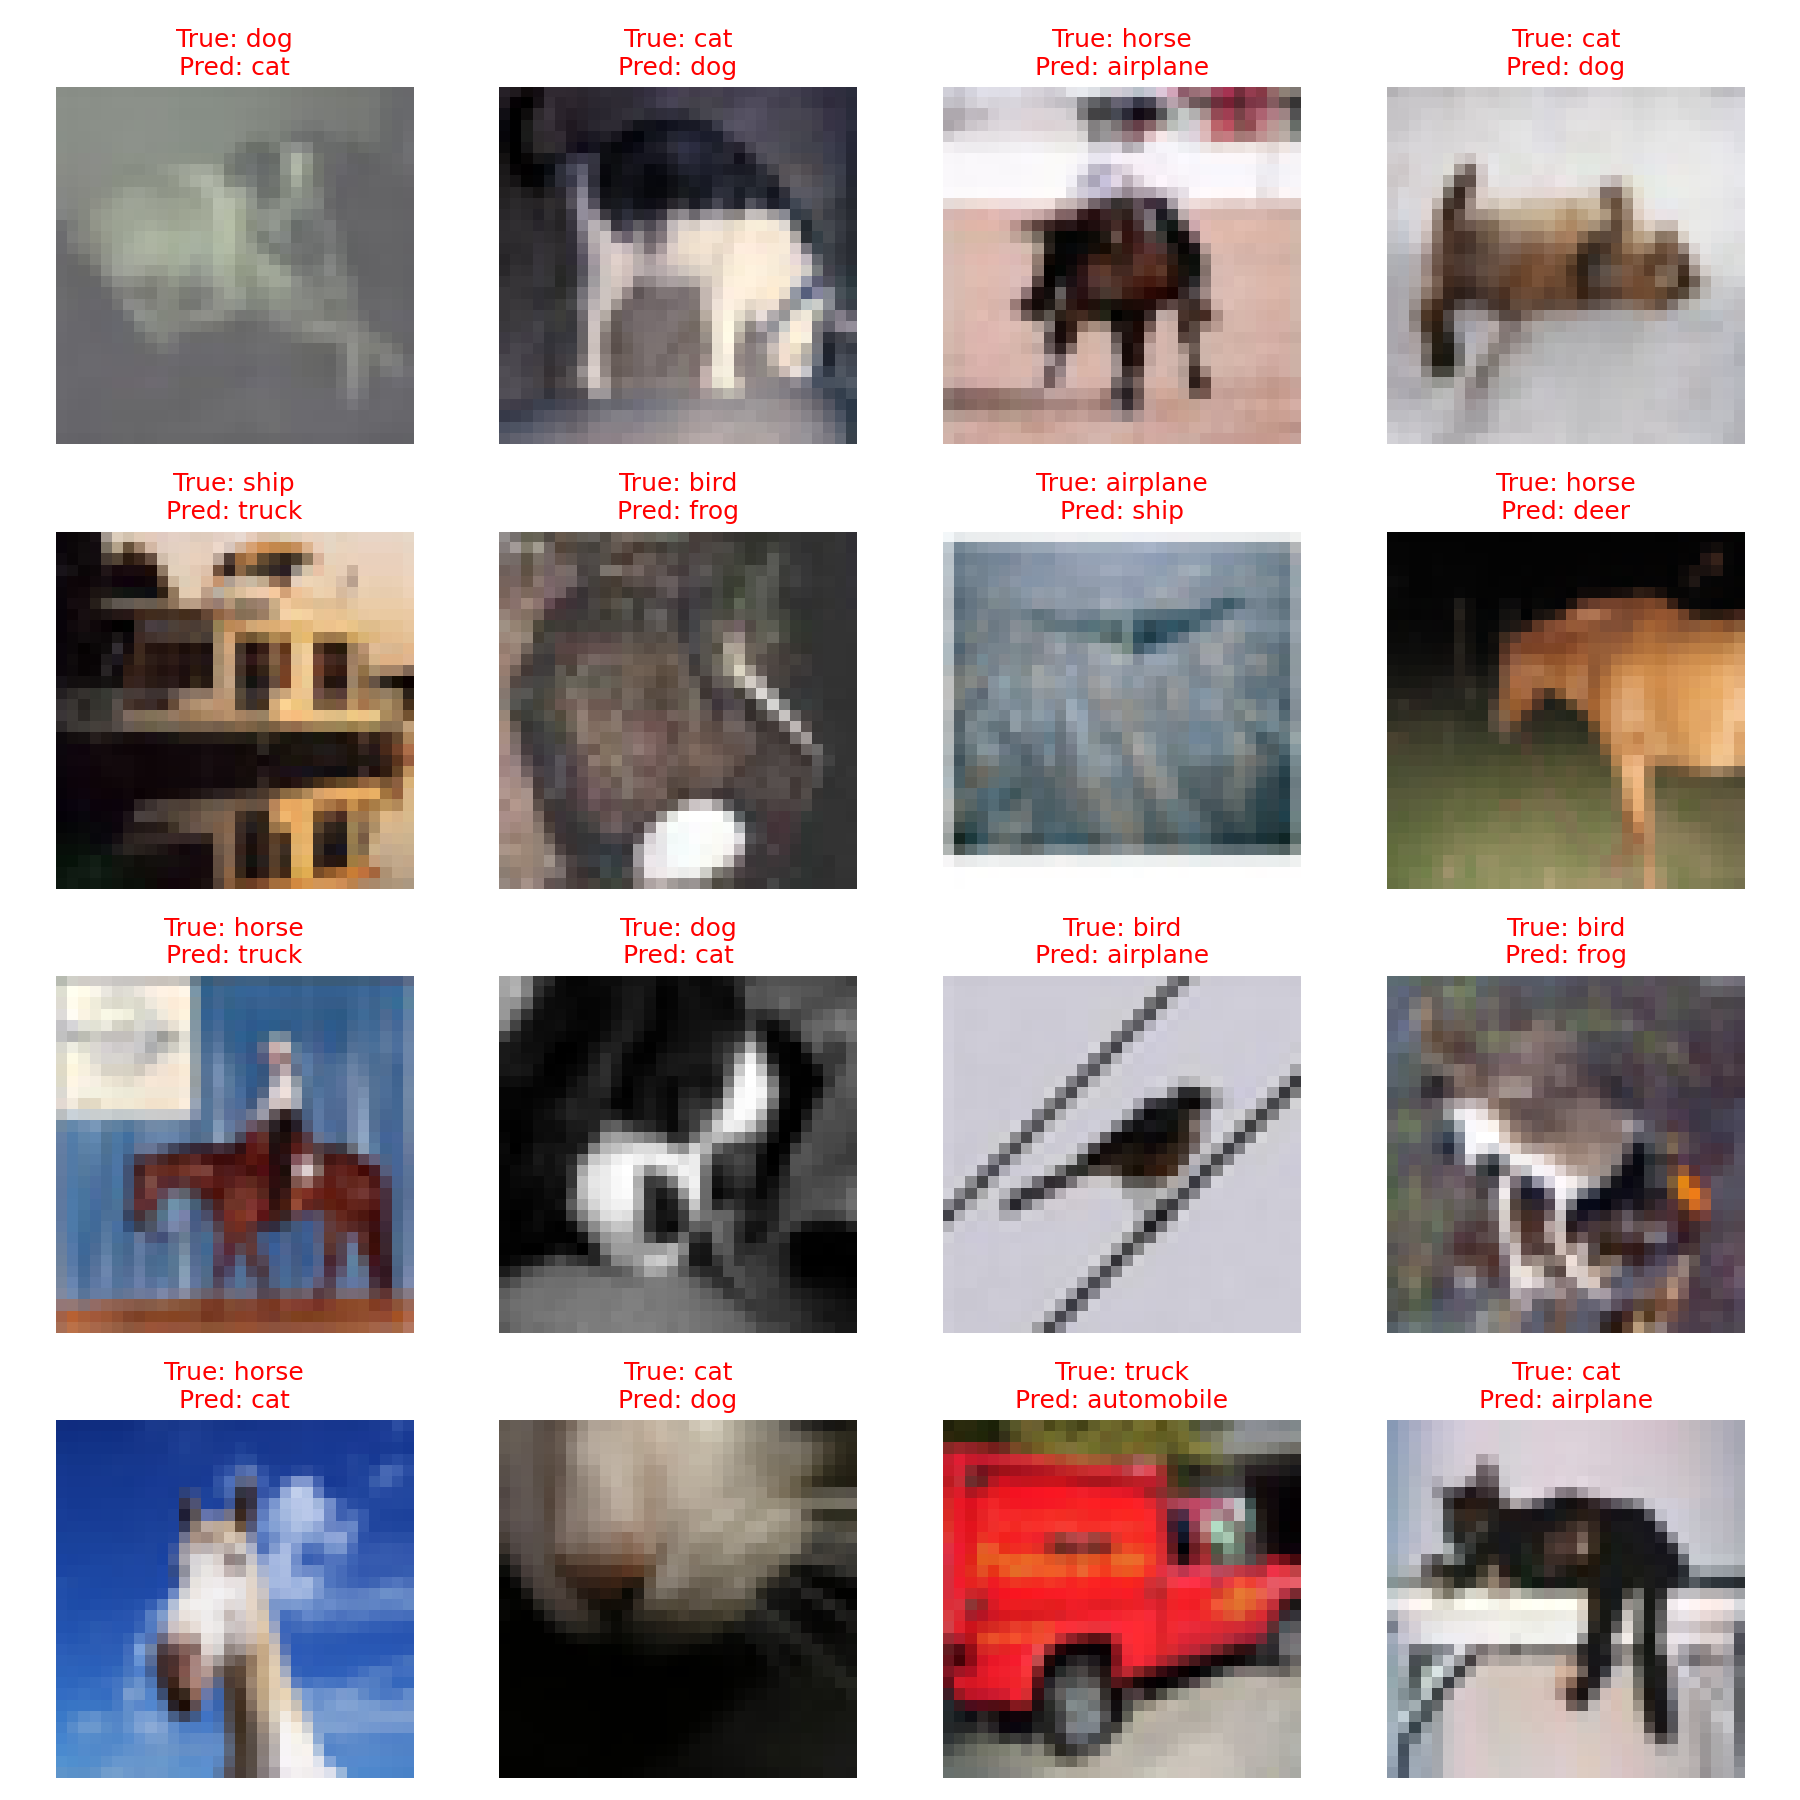
\includegraphics[width=0.85\textwidth]{codes/CIFAR10_CNN/saved/cnn_residual_relu_adam_ce_smooth_wd0.0001_wid1.0/cnn_residual_relu_adam_ce_smooth_wd0.0001_wid1.0_misclassified.png}
\caption{Misclassified examples with true and predicted labels.}
\label{fig:misclassified}
\end{figure}

\subsubsection{Comparison Across Experiments}

Figure~\ref{fig:comparisons} consolidates the key ablation results. Increasing width (a) consistently improves accuracy. Among activations (b), GELU slightly edges out ReLU and LeakyReLU. For loss functions (c), label smoothing provides a noticeable boost. Between optimizers (d), Adam converges faster and to a higher accuracy than Momentum SGD.

\begin{figure}[H]
\centering
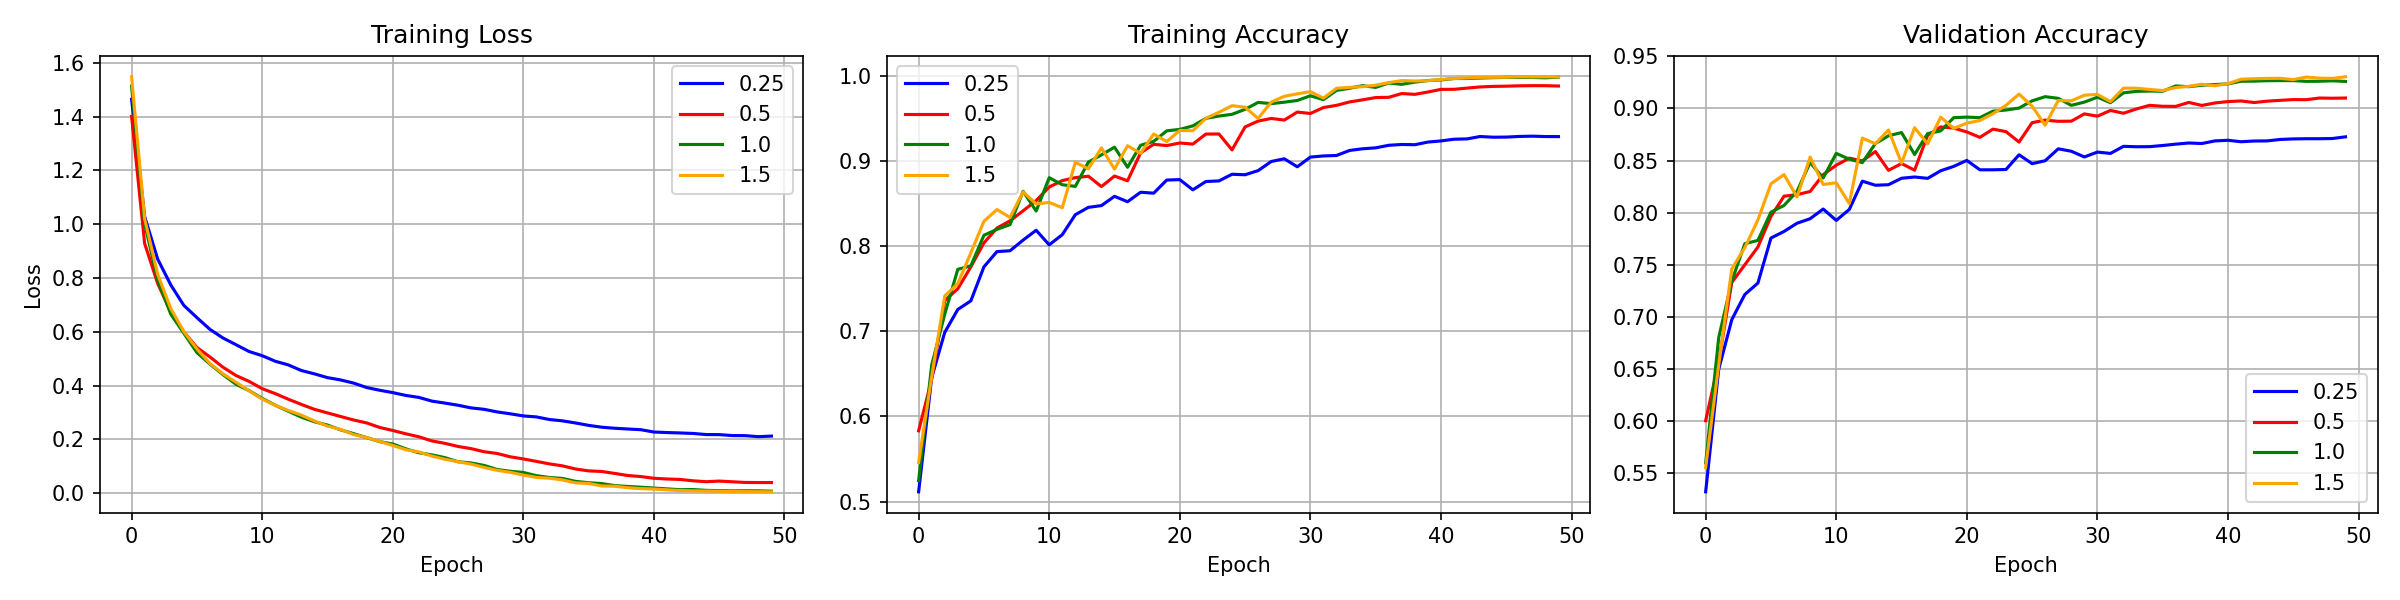
\includegraphics[width=0.48\textwidth]{codes/CIFAR10_CNN/saved/compare_width.png}\hfill
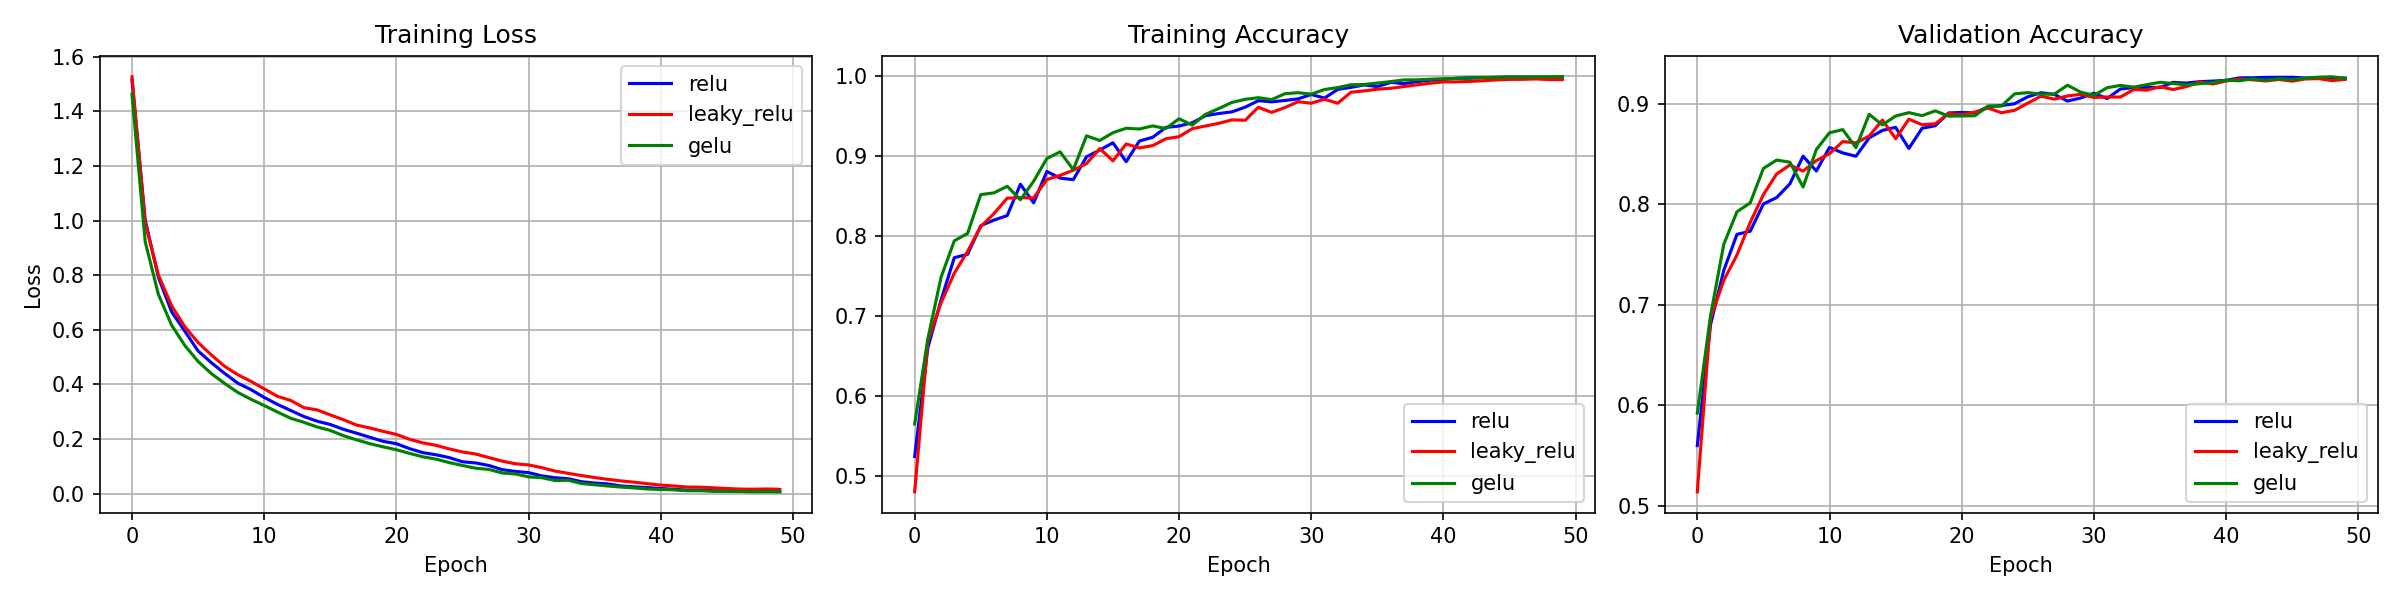
\includegraphics[width=0.48\textwidth]{codes/CIFAR10_CNN/saved/compare_act.png}
\vspace{4pt}
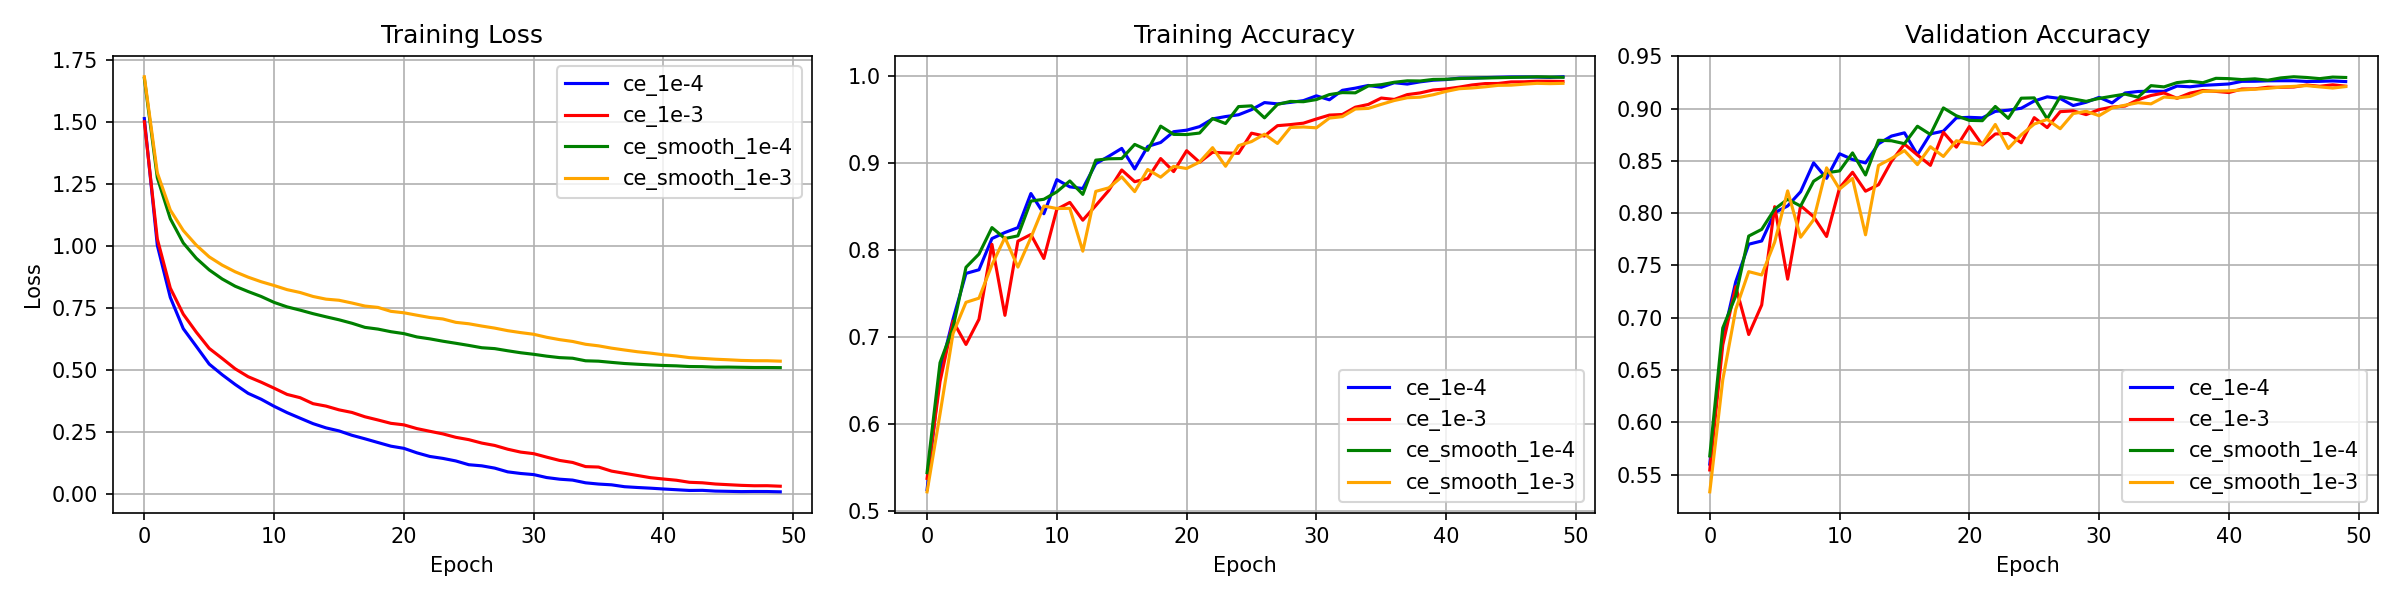
\includegraphics[width=0.48\textwidth]{codes/CIFAR10_CNN/saved/compare_loss_func.png}\hfill
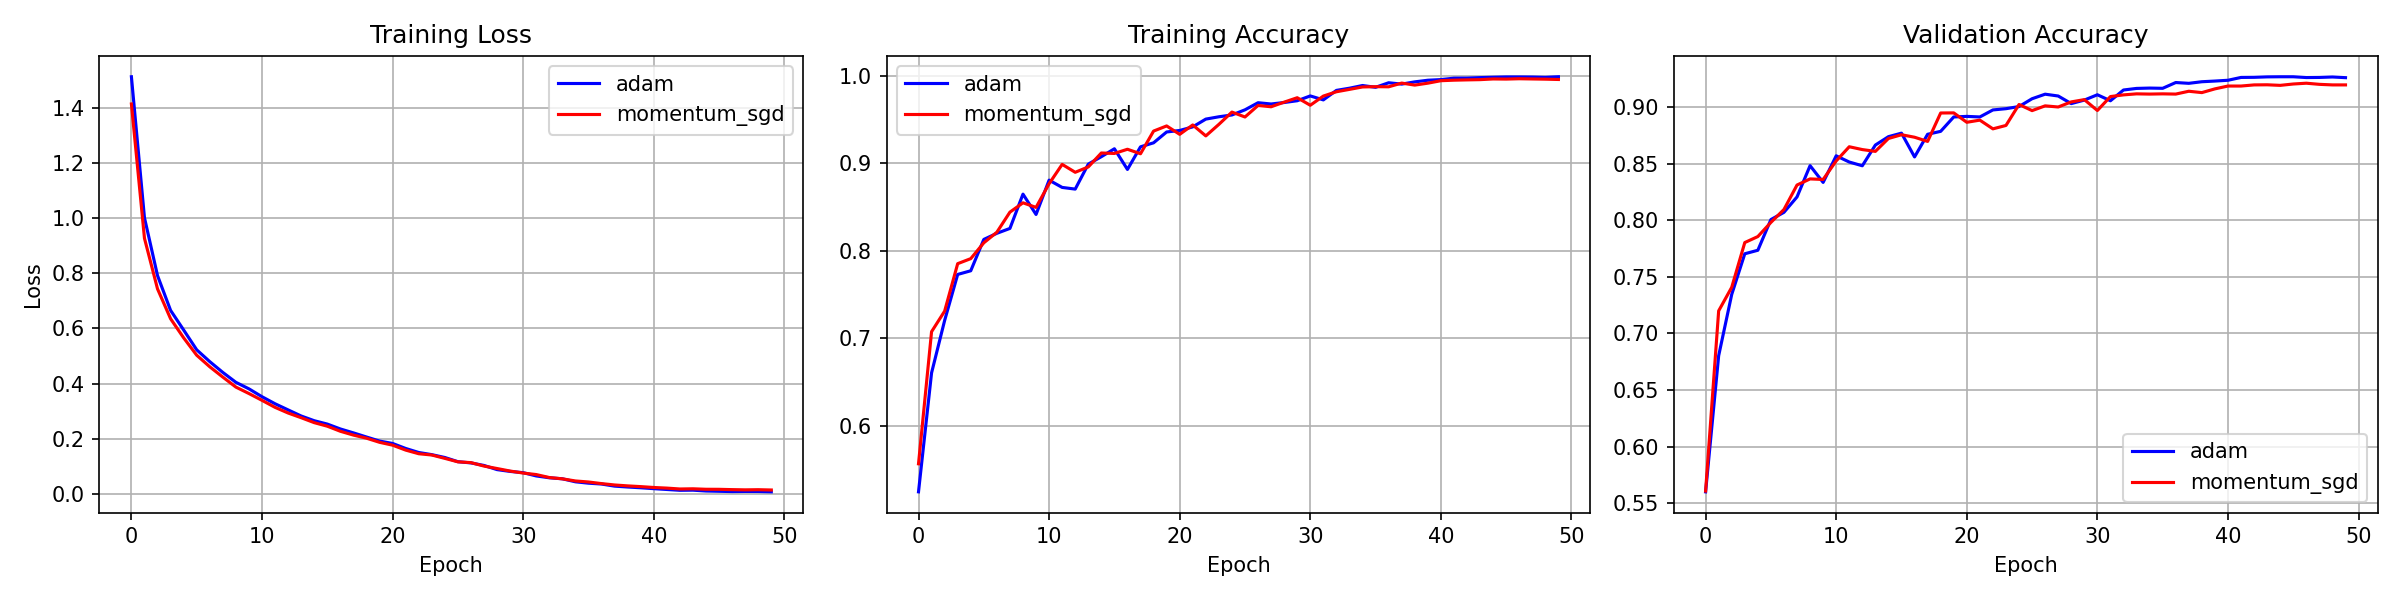
\includegraphics[width=0.48\textwidth]{codes/CIFAR10_CNN/saved/compare_optim.png}
\caption{Comparison of key experiments. (a) Width variants. (b) Activation functions. (c) Loss functions. (d) Optimizers.}
\label{fig:comparisons}
\end{figure}


% ============================================================
% 2. Batch Normalization
% ============================================================
\section{Batch Normalization}
\label{sec:bn}

Batch Normalization (BN)~\cite{ioffe2015batch} is a technique that normalizes layer inputs to have zero mean and unit variance within each mini-batch, followed by a learned affine transformation. For a convolutional network, BN is applied per-channel across all spatial locations and batch examples:

\begin{equation}
O_{b,c,x,y} \leftarrow \gamma_c \frac{I_{b,c,x,y} - \mu_c}{\sqrt{\sigma_c^2 + \epsilon}} + \beta_c
\end{equation}

where $\mu_c = \frac{1}{|B|}\sum_{b,x,y} I_{b,c,x,y}$ and $\sigma_c^2 = \frac{1}{|B|}\sum_{b,x,y} (I_{b,c,x,y} - \mu_c)^2$.

In this section, we investigate both the empirical benefits of BN and the theoretical reasons behind its effectiveness, following the framework of Santurkar et al.~\cite{santurkar2018batch}.

\subsection{VGG-A with and without Batch Normalization}

We compare VGG-A~\cite{simonyan2014very} models with and without BN on CIFAR-10. The VGG-A architecture consists of 8 convolutional layers (organized in 5 stages) followed by 3 fully-connected layers. In the BN variant (VGG\_A\_BatchNorm), we insert a BatchNorm layer after every convolutional layer and after the first two fully-connected layers. A VGG\_A\_Dropout variant is also implemented, which adds Dropout before each fully-connected layer.

All models are trained using the Adam optimizer with learning rate $10^{-3}$ and CrossEntropyLoss.

\subsection{How Does Batch Normalization Help Optimization?}

Recent work by Santurkar et al.~\cite{santurkar2018batch} demonstrates that BN's primary benefit lies in reparameterizing the optimization problem to make the loss landscape significantly smoother. We conduct three quantitative experiments to verify this claim.

\subsubsection{Experiment 1: Loss Landscape (Lipschitzness)}

\textbf{Motivation:} A smoother loss landscape implies that the loss function is more Lipschitz---i.e., its rate of change is bounded. BN should reduce the variation in loss values across different training trajectories.

\textbf{Method:} We train four VGG-A models (with BN) and four VGG-A models (without BN) using learning rates $\{10^{-3}, 2\times10^{-3}, 10^{-4}, 5\times10^{-4}\}$. At each training step, we record the per-step loss across all four learning rates and construct a band defined by the maximum and minimum loss values. A narrower band indicates greater stability to the choice of learning rate, and hence a smoother landscape.

Figure~\ref{fig:loss_landscape} shows the results. The BN model exhibits a markedly narrower loss band (blue) compared to the model without BN (red), especially during the early stages of training. This confirms that BN makes the loss landscape more Lipschitz, reducing sensitivity to the step size.

\begin{figure}[H]
\centering
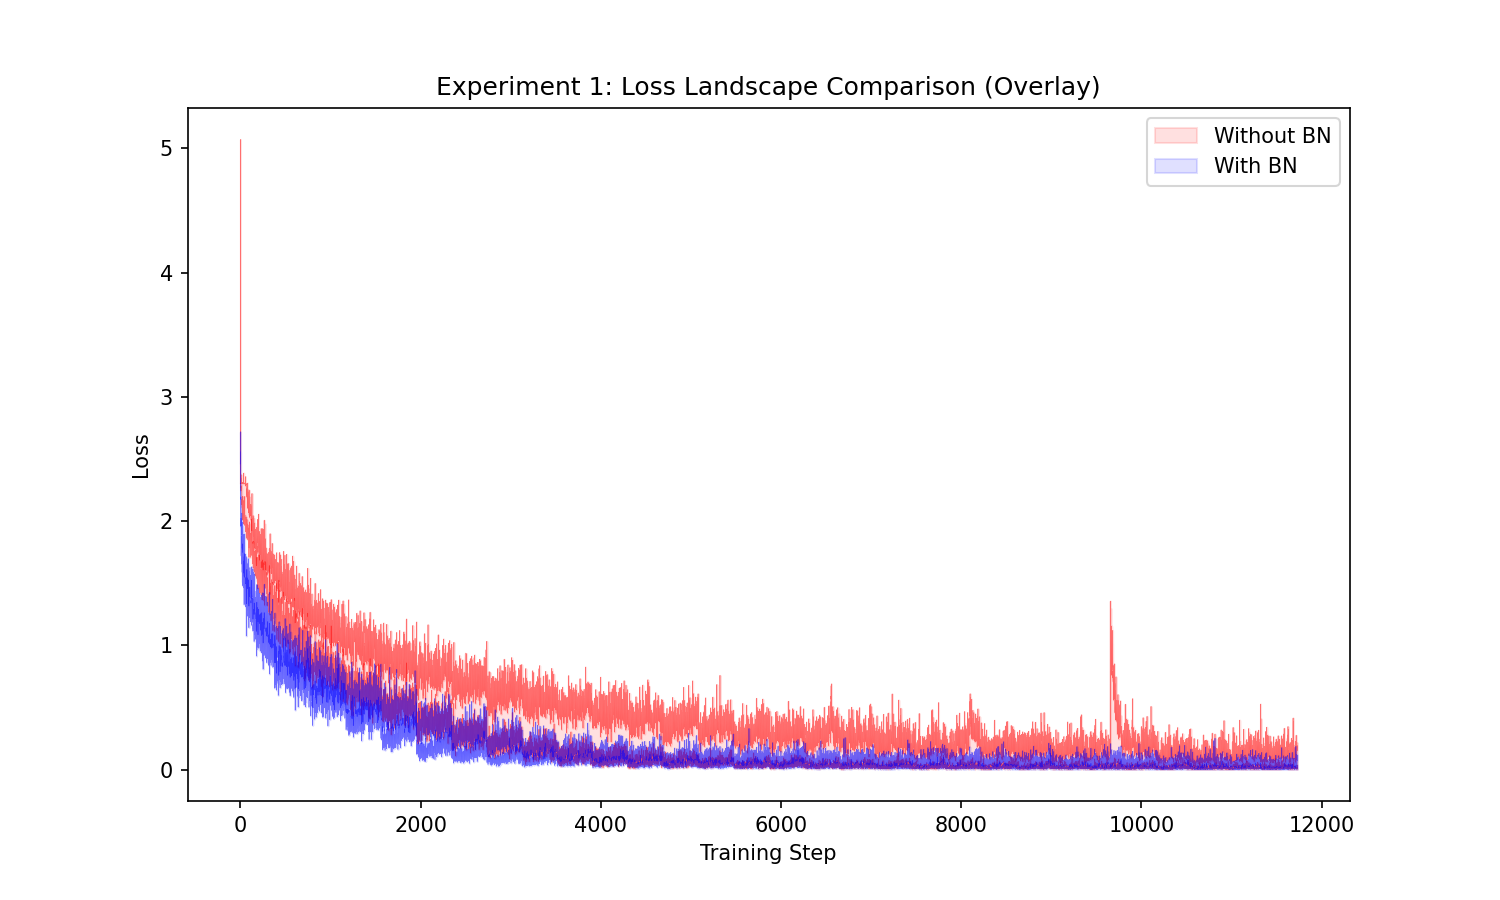
\includegraphics[width=0.95\textwidth]{codes/VGG_BatchNorm/reports/figures/exp1_loss_landscape_overlay.png}
\caption{Loss landscape comparison: VGG-A with BN (blue) vs. without BN (red). The shaded regions represent the min-max loss band across four learning rates. BN significantly narrows the loss variation.}
\label{fig:loss_landscape}
\end{figure}

\subsubsection{Experiment 2: Gradient Predictiveness}

\textbf{Motivation:} Gradient-based optimization relies on the first-order Taylor approximation:
\begin{equation}
L(\theta - \eta \nabla L(\theta)) \approx L(\theta) - \eta \|\nabla L(\theta)\|^2
\end{equation}
The accuracy of this linear approximation---termed \textit{gradient predictiveness}---determines how reliably gradient steps improve the loss. A smoother landscape yields more predictive gradients.

\textbf{Method:} At multiple checkpoints during training, we fix a batch of data and compute the predicted loss change $-\eta\|\nabla L\|^2$ versus the actual loss change $L(\theta - \eta\nabla L) - L(\theta)$ for a range of step sizes $\eta \in [0.1, 15.8]$. The prediction error $|\Delta L_{\text{actual}} - \Delta L_{\text{pred}}|$ quantifies gradient predictiveness.

Figure~\ref{fig:grad_predictiveness} (left) shows that at the final epoch, the BN model consistently achieves lower prediction errors across all step sizes. The right panel shows the ratio $|\text{actual}/\text{predicted}|$; the BN curve stays closer to 1.0 (perfect prediction), indicating that the local linear approximation remains valid over a wider range of step sizes.

\begin{figure}[H]
\centering
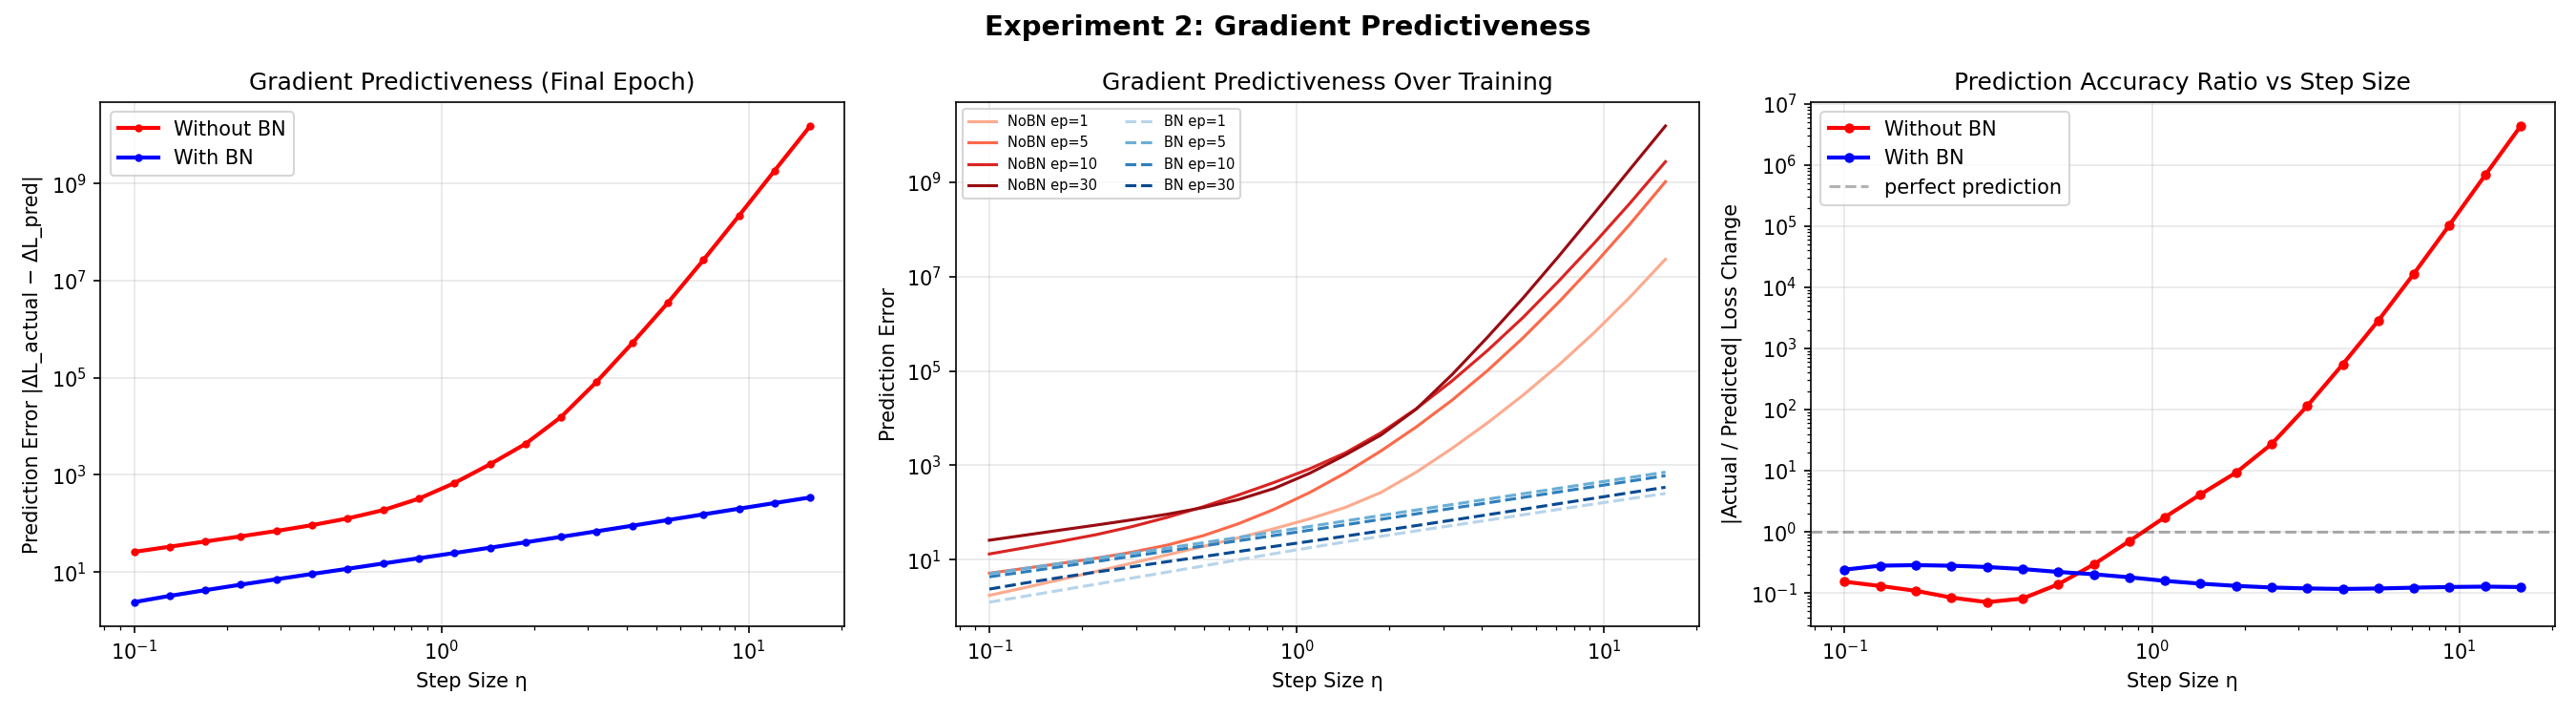
\includegraphics[width=0.95\textwidth]{codes/VGG_BatchNorm/reports/figures/exp2_gradient_predictiveness.png}
\caption{Gradient predictiveness comparison. Left: Prediction error vs.\ step size at the final epoch. Center: Error evolution across training epochs. Right: Ratio of actual to predicted loss change. BN (blue) consistently outperforms the non-BN model (red).}
\label{fig:grad_predictiveness}
\end{figure}

\subsubsection{Experiment 3: $\alpha$-Smoothness (Maximum Gradient Difference)}

\textbf{Motivation:} $\alpha$-smoothness measures how much the gradient changes under small perturbations in parameter space. A function is $\alpha$-smooth if:
\begin{equation}
\|\nabla L(\theta + \delta d) - \nabla L(\theta)\| \leq \alpha \|\delta d\|
\end{equation}
Smaller $\alpha$ implies a more predictable and stable optimization trajectory.

\textbf{Method:} For perturbation distances $\delta \in [0.01, 3.98]$, we sample 5 random unit directions $d$, compute $\|\nabla L(\theta + \delta d) - \nabla L(\theta)\|$, and average the results. We repeat this at multiple training checkpoints.

Figure~\ref{fig:alpha_smoothness} (left) shows the final-epoch comparison: the BN model exhibits consistently smaller gradient differences across all perturbation distances. The right panel tracks the effective smoothness constant $L$ over training; the BN model maintains a lower smoothness constant, and the gap widens as training progresses---suggesting that BN's smoothing effect compounds over the course of optimization.

\begin{figure}[H]
\centering
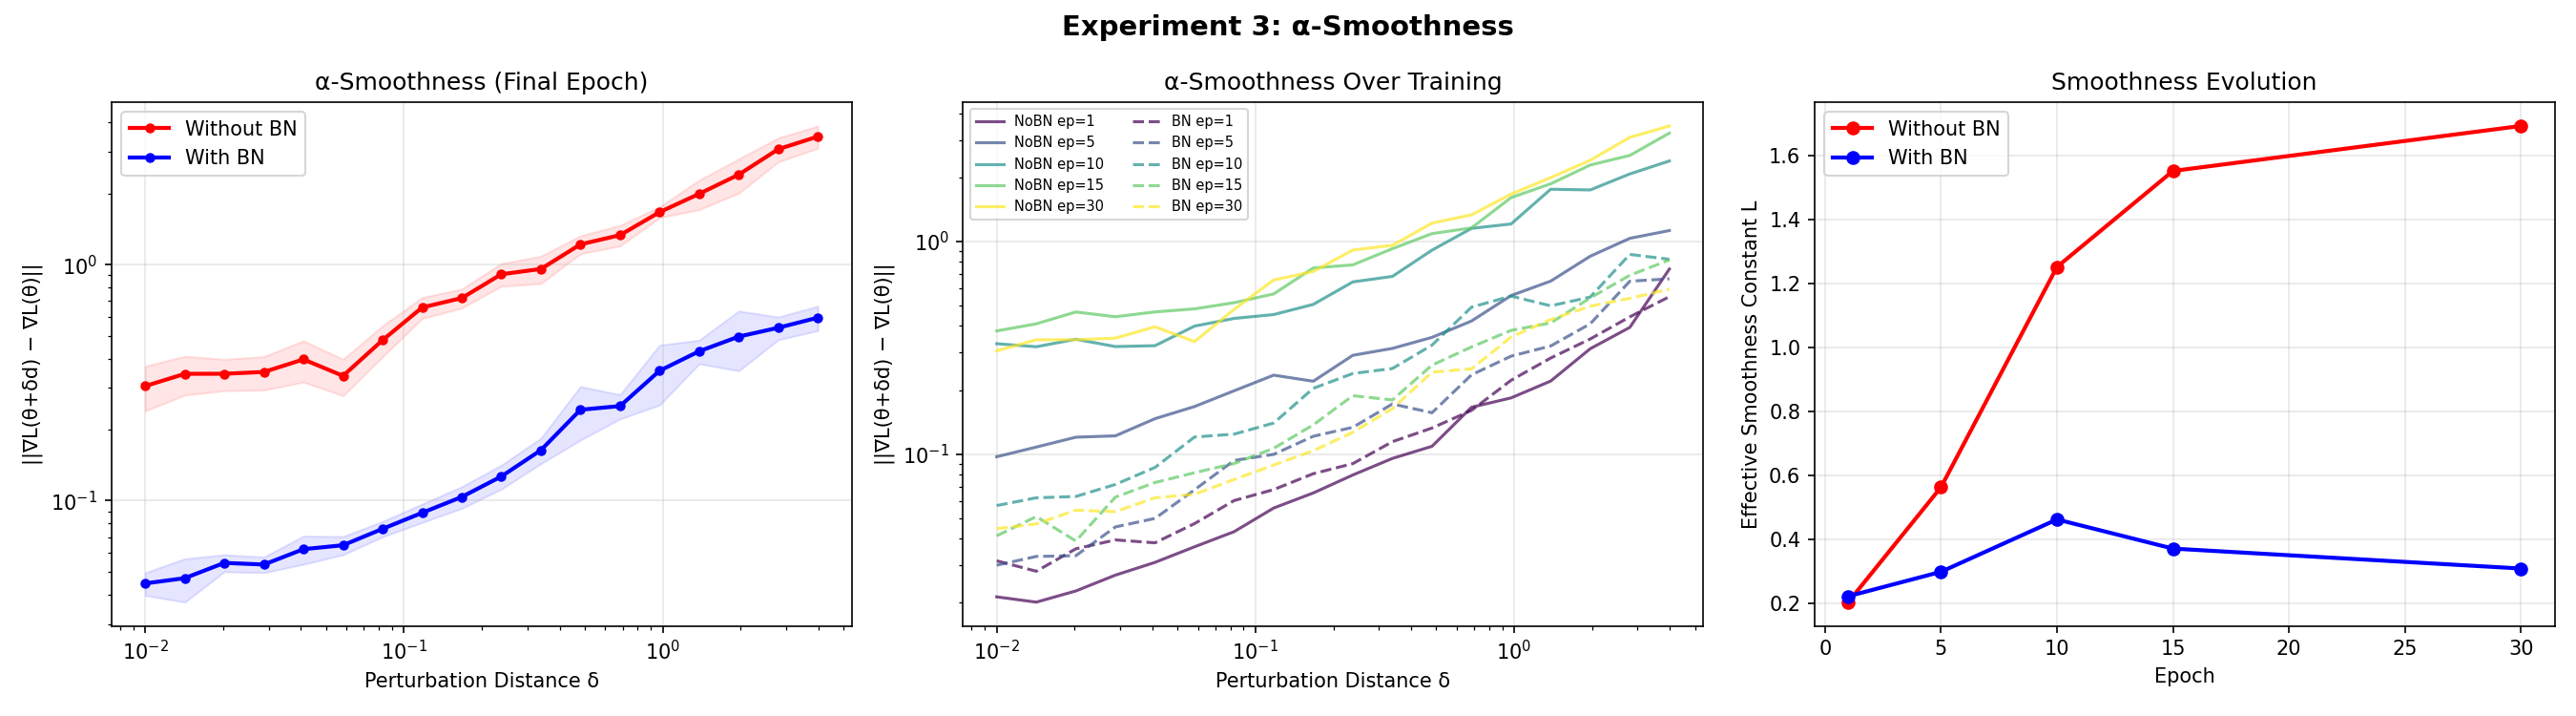
\includegraphics[width=0.95\textwidth]{codes/VGG_BatchNorm/reports/figures/exp3_alpha_smoothness.png}
\caption{$\alpha$-smoothness comparison. Left: Gradient difference vs.\ perturbation distance at the final epoch. Center: Evolution across training epochs. Right: Effective smoothness constant over training. BN (blue) shows smaller gradient variation.}
\label{fig:alpha_smoothness}
\end{figure}

\subsubsection{Summary of BN Analysis}

Summarizing these three experiments, the key findings are:

\begin{enumerate}[nosep]
    \item \textbf{Loss Landscape:} BN narrows the loss variation band across different learning rates, confirming improved Lipschitzness.
    \item \textbf{Gradient Predictiveness:} BN yields lower prediction errors, meaning the first-order gradient approximation is more reliable---enabling larger, more confident update steps.
    \item \textbf{$\alpha$-Smoothness:} BN reduces gradient variation under parameter perturbations, leading to more stable and consistent gradient updates.
\end{enumerate}

Together, these results support the conclusion that BN reparameterizes the underlying optimization problem, making the loss landscape significantly smoother and enabling faster, more stable training of deep neural networks.


% ============================================================
% Conclusion
% ============================================================
\section{Conclusion}

In this project, we conducted a comprehensive empirical study of convolutional neural network training on CIFAR-10 and a systematic analysis of Batch Normalization.

For Part~1, we adopted the CNN\_Residual architecture—which integrates all required components (convolutional, pooling, fully-connected layers, activations) and two optional components (BatchNorm, residual connections) into a single unified design. Using a controlled-variable methodology, we systematically varied network width, activation functions, loss functions with regularization, and optimizers to isolate each parameter's effect. The optimal configuration achieves \textbf{93.04\% test accuracy} with ReLU, Adam, and label smoothing at width=1.0 (3.0M parameters). Key findings include: (1)~label smoothing provides the single largest improvement (+0.38\%), (2)~Adam outperforms Momentum SGD by 0.57\%, (3)~GELU slightly edges out ReLU but the margin is negligible, and (4)~increasing width yields diminishing returns beyond width=1.0.

For Part~2, we demonstrated through three quantitative experiments that Batch Normalization smooths the optimization landscape. Compared to standard VGG-A, the BN-augmented model exhibits: (1) reduced loss variation across learning rates (improved Lipschitzness), (2) more accurate first-order gradient predictions (improved gradient predictiveness), and (3) smaller gradient changes under parameter perturbations (improved $\alpha$-smoothness). These findings align with and provide experimental validation for the theoretical framework proposed in recent literature~\cite{santurkar2018batch}.


% ============================================================
% References
% ============================================================
\begin{thebibliography}{9}

\bibitem{krizhevsky2009learning}
A.~Krizhevsky and G.~Hinton,
\emph{Learning Multiple Layers of Features from Tiny Images},
Technical Report, University of Toronto, 2009.

\bibitem{ioffe2015batch}
S.~Ioffe and C.~Szegedy,
``Batch Normalization: Accelerating Deep Network Training by Reducing Internal Covariate Shift,''
in \emph{Proc. ICML}, 2015.

\bibitem{santurkar2018batch}
S.~Santurkar, D.~Tsipras, A.~Ilyas, and A.~Madry,
``How Does Batch Normalization Help Optimization?,''
in \emph{Proc. NeurIPS}, 2018.

\bibitem{simonyan2014very}
K.~Simonyan and A.~Zisserman,
``Very Deep Convolutional Networks for Large-Scale Image Recognition,''
in \emph{Proc. ICLR}, 2015.

\bibitem{pytorch_cifar10}
PyTorch Tutorial,
``Training a Classifier (CIFAR-10),''
\url{https://pytorch.org/tutorials/beginner/blitz/cifar10_tutorial.html}.

\end{thebibliography}


\end{document}
